\chapter{Teoretične osnove}

Parametre izbrane hidroelektrarne lahko izračunamo po naslednjem algoritmu:
\begin{enumerate}[noitemsep, topsep=0pt]
	\item Pridobitev podatkov
	\item Izračun hidrološkega niza podatkov za obdobje
	\item Izračun konsumpcijske krivulje
	\item Izračun proizvodnje električne energije
\end{enumerate}


%-------------------------------------
\section{Pridobitev podatkov}
Za nadaljnje izračune potrebujemo podatke o:
\begin{itemize}[noitemsep, topsep=0pt]
	\item Dimenzijah rečne struge
	\item Naklonu in oceno Manningovega koeficienta hrapavosti rečnega korita
	\item Povprečnih dnevnih pretokih vodotoka za izbrano obdobje
\end{itemize}

Podatke o dimenzijah rečne struge lahko pridobimo z meritvami ali pa dimenzije ocenimo na podlagi ortofoto posnetkov. Naklon se lahko oceni s pomočjo spletne aplikacije Geopedija, kjer so vneseni podatki o višinski razliki izbranih točk $\Delta h$ rečne struge in razdalje med točkami $L$. Naklon rečne struge izračunamo po enačbi:
\begin{align}
 I = \dfrac{100\Delta h}{L} [\%]
\end{align}


  Manningov koeficient hrapavosti rečnega korita $ng$ se lahko oceni izkustveno na terenu s pomočjo priročnikov ali pa z umerjanjem na podlagi podatkov o nivojih vode in pretokih. Odvisen od naslednjih 7 faktorjev \cite{VenTeChow}:
 \begin{enumerate}[noitemsep, topsep=0pt]
 	\item Hrapavosti površine ostenja
 	\item Zaraščenosti rečnega korita
 	\item Neregularnosti oblike rečnega korita
 	\item Meandriranja rečne struge
 	\item Zamašitve struge s plavinami 
 	\item Oblike in velikosti rečnega korita
 	\item Polnosti korita
 \end{enumerate}
 

 
 
  Podatke o pretokih slovenskih vodotokov lahko pridobimo iz arhiva, ki se nahaja na spletni strani agencije Republike Slovenije za okolje (ARSO). V primeru da iščemo pretok za manjši vodotok, obstaja velika verjetnost da podatki o pretokih ne obstajajo. V tem primeru lahko pretok vodotoka ocenimo s pomočjo meritev višine gladine vode in dimenzij struge, ocene Manningovega koeficienta hrapavosti in naklona struge. S pomočjo Manningove enačbe opisane v poglavju~\ref{sec:teorija_trapeznaMetoda} in ocenjenih členov enačbe dobimo končno ocenjeno vrednost pretokov za posamezno obdobje meritev.




%------------------------------------------------
\section{Izračun hidrološkega niza podatkov}
%TODO: FIXME -> izboljšaj
Iz arhiva lahko izvozimo podatke o povprečnih dnevnih pretokih v csv (comma separated values) obliki. Iz podatkov lahko za vsak mesec obdobja izračunamo povprečni mesečni pretok. Če mesečne pretoke povprečimo za vsa leta izbranega obdobja lahko navedene povprečne mesečne pretoke obdobja prikažemo na hidrogramu. Prav tako se lahko določi mokro in suho leto obdobja, ki ju primerjamo z povprečnimi mesečnimi pretoki.



%------------------------------------------------
\section{Izračun konsumpcijske krivulje}
Konsumpcijska krivulja je graf, ki predstavlja višino gladine spodnje vode v rečni strugi v odvisnosti od pretoka vode skozi turbine hidroelektrarne. Graf konsumpcijske krivulje potrebujemo za določitev višinske razlike $dh$ med spodnjo in zgornjo vodo v odvisnosti od pretoka vode skozi turbine hidroelektrarne. Višinsko razliko $dh$ potrebujemo za določitev moči hidroelektrarne v zadnjem koraku algoritma opisanega v tem poglavju.



%-------------------------------------------------
\subsection{Izračun konsumpcijske krivulje za pravokotne in trapezne struge} \label{sec:teorija_trapeznaMetoda}
Za izračun konsumpcijske krivulje potrebujemo pretok vodotoka v odvisnosti od višine gladine vode $h$ v strugi. Gladina vode $h$ poteka od dna struge do maksimalne višine struge $H$. Pretok vode v strugi se za vsak cm višine $h$ izračuna po Manningovi enačbi:

\begin{ceqn}
\begin{align}
Q(h) = \dfrac{1}{ng} \sqrt{I}\dfrac{S(h)^{5/3}}{P(h)^{2/3}} \label{eq:ManningovaEnacba}
\end{align}
\end{ceqn}

Kjer je:

\begin{table}[htb!]
	\begin{tabular}{r|p{10cm}}
		Q & pretok \\
		ng & Manningov koeficient hrapavosti dna struge\\
		I & naklon struge \\
		S & ploščina prečnega profila \\
		P & dolžina omočenega oboda struga
	\end{tabular}
\end{table}



% pravokotna struga
\begin{enumerate}
	\item Pravokotna struga:
	
	\begin{figure}[ht!]
		\begin{centering}
			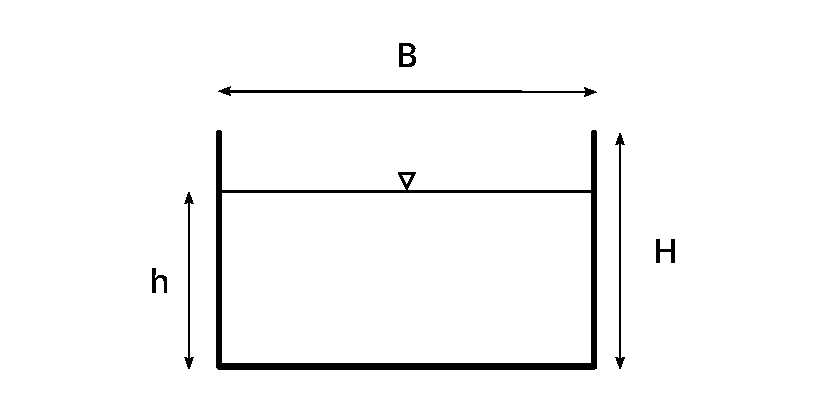
\includegraphics{slike/konsumpcijska_krivulja/rectangularChannel.pdf}		
			\caption{Prečni prerez pravokotne struge}\label{fig:pravokotna struga}
		\end{centering}
	\end{figure}
	

	Omočeni obod pravokotne struge izračunamo kot seštevek širine dna struge in dvakratne višine struge $h$.
	
	\begin{ceqn}
	\begin{equation}
	P_{p}(h) = B + 2h
	\end{equation}
	\end{ceqn}
	
	Ploščino pravokotne struge dobimo po enačbi:
	
	\begin{ceqn}
	\begin{align}
	S_{p}(h) = B \cdot h
	\end{align}
	\end{ceqn}
	
	\item Trapezna struga:
	
		\begin{figure}[ht!]
			\begin{centering}
				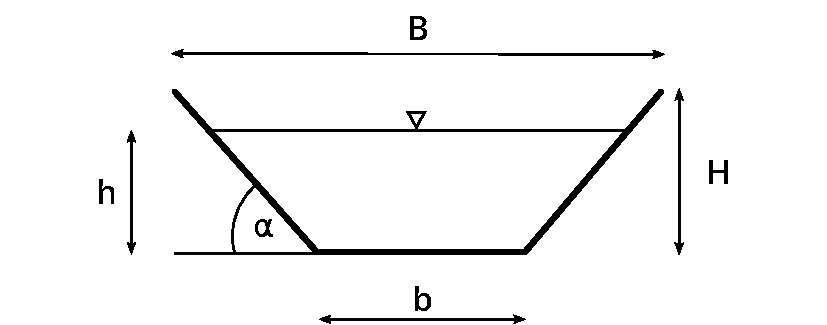
\includegraphics{slike/konsumpcijska_krivulja/trapezoidChannel.pdf}		
				\caption{Prečni prerez trapezne struge}\label{fig:trapezna struga}
			\end{centering}
		\end{figure}
	
	Omočeni obod trapezne struge izračunamo kot seštevek širine dna struge in dvakratne razdalje od roba dna struge do točke presečišča rečnega korita z gladino vode.
	
	\begin{ceqn}
	\begin{align}
	P_{t}(h) = b + 2 \cdot \sqrt{h^2 + \left(\dfrac{h} {\tan\alpha} \right)^{2}}
	\end{align}
	\end{ceqn}
	
	Ploščino trapezne struge izračunamo po enačbi:
	\begin{ceqn}
	\begin{align}
	S_{t}(h) = b \cdot h + \dfrac{h^2}{ 2\tan\alpha}
	\end{align}
	\end{ceqn}
	
\end{enumerate}



Ko poznamo vse parametre Manningove enačbe \ref{eq:ManningovaEnacba}, izračunamo pretoke vodotoka za vsak cm višine rečne struge, ki poteka od 0 do $H$ in narišemo konsumpcijsko krivuljo $h(Q)$.


\newpage
%------------------------------------------------
\section{Izračun konsumpcijske krivulje za struge poljubne oblike}\label{sec:pretokNumericnaMetoda}


Poljubno oblikovano strugo lahko popišemo s serijo točk, ki jih dodajamo v kartezijski koordinatni sistem. Za vsako točko poljubnega rečnega korita podamo x in y koordinato, za točke pa predpostavimo da so med seboj povezane z enačbo linearne funkcije. 

\begin{figure}[ht!]
	\begin{centering}
		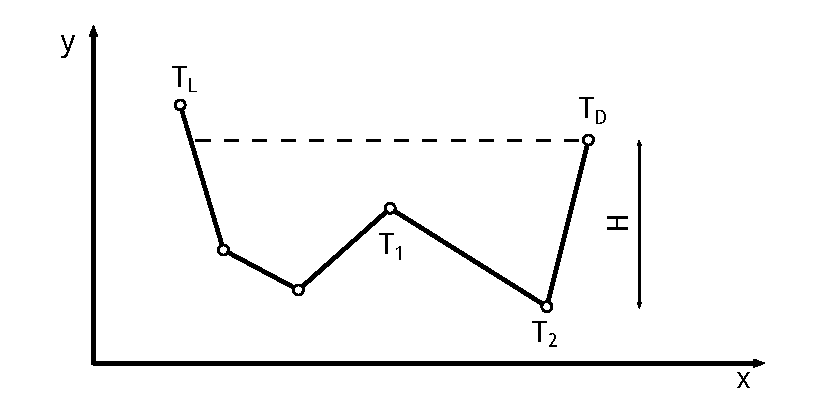
\includegraphics{slike/customChannel/customStruga.pdf}		
		\caption{Poljubno definirana struga}\label{fig:poljubnaStruga}
	\end{centering}
\end{figure}



%------------------------------------------
\subsection{Izračun višine rečnega korita}
Skrajni točki struge sta točki $T_L$ in $T_D$ na sliki \ref{fig:poljubnaStruga}. Točko na robu struge z najnižjo y koordinato označimo s $T_{Smin}$ (na sliki \ref{fig:poljubnaStruga} točka $T_D$). Najnižjo točko poljubne struge označimo s $T_{min}$ (na sliki \ref{fig:poljubnaStruga} točka $T_2$). Višina rečnega korita $H$ je definirana kot razdalja med točkama $T_{Smin}$ in $T_{min}$.




\subsection{Določitev parametrov odseka}

Program razdeli podano strugo na odseke po dve točki $T_1$ ($x_1$, $y_1$) in $T_2$ ($x_2$, $y_2$). Za podan odsek se najprej določi enačba linearne funkcije. 

\begin{ceqn}
\begin{align}
f(x) = kx + n \label{eq:enacba_linearnafunkcija}
\end{align}
\end{ceqn}

Naklon funkcije k se izračuna po formuli: 

\begin{ceqn}
\begin{align}
k = \dfrac{y_2 - y_1}{x_2 - x_1}
\end{align}
\end{ceqn}



\begin{figure}[ht]
	\begin{centering}
		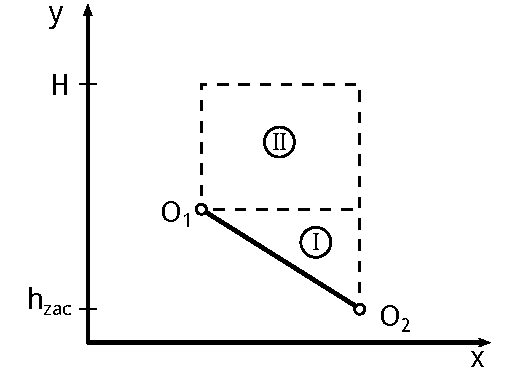
\includegraphics{slike/customChannel/odsek.pdf}
		\caption{Izbrani odsek struge} \label{fig:odsekStruge}
	\end{centering}
\end{figure}




Če v enačbo linearne funkcije \ref{eq:enacba_linearnafunkcija} vstavimo izračunan k in koordinate točke $T_1$, lahko izračunamo iskani $n$ in s tem je določena enačba linearne funkcije $f(x)$ med dvema točkama, ki jo potrebujemo za nadaljnje izračune. 



% določitev ploščine posameznega kosa
Za vsak odsek dveh točk se najprej določi najnižja točka odseka $T_{zac}$, na sliki \ref{fig:odsekStruge} označena kot točka $O_2$. Y koordinata točke $T_{zac}$ nam predstavlja začetno višino odseka $h_{zac}$. Razdaljo med začetno višino odseka $h_{zac}$ in končno gladino struge $H$ označimo z $dh$.

% explain
Od $h_{zac}$ do končne višine rečnega korita H za vsak cm po višini določimo presečišče $P_1$ prej izračunane funkcije $f(x)$ s horizontalno ravnino $g$, ki predstavlja gladino vode pri trenutni višini $h$.


\begin{figure}[ht!]
	\begin{centering}
		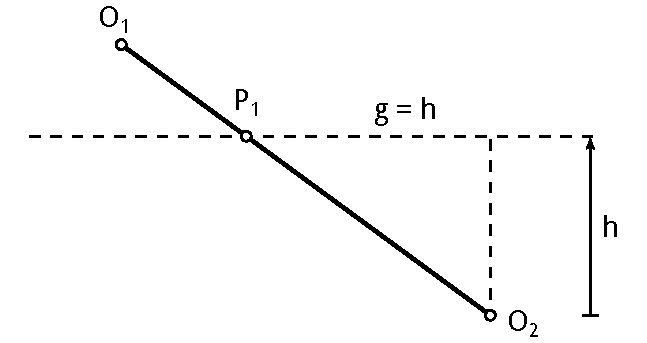
\includegraphics{slike/customChannel/odsek_detajl.pdf}
		\caption{Detajl odseka struge}
	\end{centering}
\end{figure}



Ko imamo določeno presečišče $P_1$ gladine vode s funkcijo $f(x)$ med točkama odseka, lahko izračunamo dolžino omočenega oboda struge in ploščino lika ki ga oklepajo funkcija odseka, navidezna gladina vode $g$ in najnižja točka odseka $T_{zac}$ na sliki \ref{fig:odsekStruge} označena z $O_2$.


\begin{enumerate}
	\item V primeru da se presečišče $P1$ odseka nahaja v območju med točkama $O_1$ in $O_2$, dolžino omočenega oboda določimo po Pitagorovem izreku kot:
	
	%\begin{equation}
	%P = \sqrt{(T_{zac}x - P_1x)^{2} + (T_{zac}y - P_1y)^{2}}
	%\end{equation}
	
	\begin{ceqn}
		\begin{align}
		P = \sqrt{(T_{zac}x - P_1x)^{2} + (T_{zac}y - P_1y)^{2}}
		\end{align}
	\end{ceqn}
	
	
	ploščino področja ki ga oklepajo horizontalna ravnina s presečiščem $P_1$ in najnižjo točko odseka $T_{zac}$ pa določimo kot ploščino trikotnika (področje I na sliki~\ref{fig:odsekStruge}) po formuli:
	
	\begin{ceqn}
	\begin{align}
	S = \dfrac{|T_{zac}x - P_1x| \cdot |T_{zac}y - P_1y|}{2}
	\end{align}
	\end{ceqn}
	
	
	\item V primeru, da se presečišče $P1$ nahaja izven območja točk $O_1$ in $O_2$ pa se dolžina omočenega oboda izračuna kot razdalja med točkama $O_1$ in $O_2$ po Pitagorovem izreku:
	
	\begin{ceqn}
	\begin{align}
	P = \sqrt{ (O_1x - O_2x)^{2} + (O_1y - O_2y)^{2}}
	\end{align}
	\end{ceqn}
	
	Ploščina pa se določi kot seštevek ploščin območij I in II na sliki \ref{fig:odsekStruge}.
	
	\begin{ceqn}
	\begin{align}
	S = S_I + S_{II}
	\end{align}
	\end{ceqn}
	
	Pri čemer sta $S_I$ in $S_{II}$ enaka:
	

	\begin{ceqn}
	\begin{align}
	S_I =\dfrac{ (O_2y - O_1y) *  (O_2x - O_1x)}{2}
	\end{align}
	
	\begin{align}
	S_{II} = (O_2x - O_1x) * (H - O_1y)
	\end{align}
	\end{ceqn}

	
	
	
	
\end{enumerate}


Za določitev končne dolžine omočenih obodov pri iskani višini $h$ moramo sešteti vse omočene obode odsekov pri iskani višini $h$.
\begin{ceqn}
\begin{align}
P(h) = P_1(h) + P_2(h) + P_3(h) + ... + P_{n-1}(h) + P_n(h)
\end{align}
\end{ceqn}



Za določitev končnih vrednosti ploščin likov $S$ pri iskani višini $h$, moramo sešteti ploščine $S$ pri iskani višini $h$ za vse odseke točk rečne struge, to so vse točke med $T_L$ in $T_D$ na sliki~\ref{fig:poljubnaStruga}

\begin{ceqn}
\begin{align}
S(h) = S_1(h) + S_2(h) + S_3(h) + ... + S_{n-1}(h) + S_n(h)
\end{align}
\end{ceqn}



% TODO: kako izračunamo končni pretok za izris konsumpcijske krivulje.


Za izris konsumpcijske krivulje potrebujemo podatke o pretokih v odvisnosti od višine vode v strugi. Za vsak odsek struge imamo na voljo podatke o ploščini prečnega profila struge in omočenega oboda dna struge v odvisnosti od višine vode v strugi. Pretoke za vsak cm višine vode v strugi izračunamo po Manningovi enačbi \ref{eq:ManningovaEnacba}


Ko imamo posamezne pretoke po višinah za vse odseke izračunane, jih medsebojno seštejemo in dobimo končne vrednosti pretokov:

\begin{ceqn}
\begin{align}
Q(h) = Q_1(h) + Q_2(h) + Q_3(h) + ... + Q_{n-1}(h) + Q_n(h)
\end{align}
\end{ceqn}

Sledi izris konsumpcijske krivulje $h(Q)$.


%TODO: screenshot konsumpcijske krivulje


\newpage



\section{Izračun proizvodnje električne energije}
Za določitev končne proizvodnje električne energije potrebujemo razliko med koto zgornje vode (vode v rezervoarju) in koto spodnje vode, ki jo določimo iz grafa konsumpcijske krivulje izračunanega za izbrano strugo.

\begin{figure}[ht!]
	\begin{centering}
		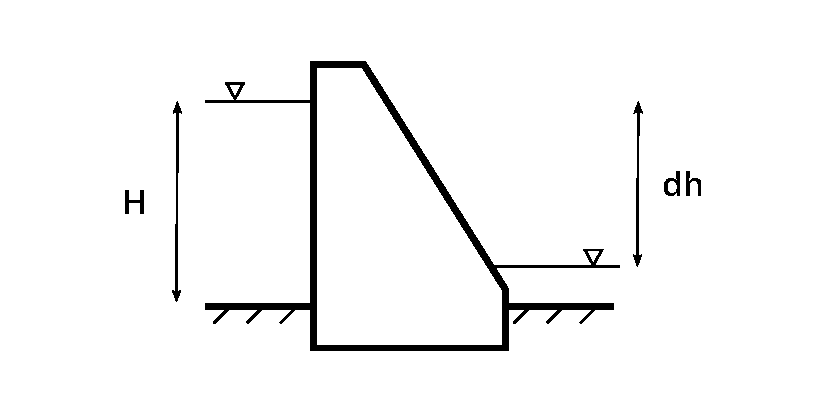
\includegraphics{slike/electricityProduction/powerplant_crossSection.pdf}
		\caption{Prečni prerez hidroelektrarne}
	\end{centering}
\end{figure}

Ker računamo proizvodnjo električne energije za pretočne hidroelektrarne, predpostavimo da je kota zgornje vode konstantna na višini $H$. Koto spodnje vode določimo iz prej izračunane konsumpcijske krivulje, kjer določimo višino spodnje vode v strugi za dani povprečni mesečni pretok skozi turbino hidroelektrarne. V primeru da se pretok skozi turbino hidroelektrarne nahaja med dvema točkama pretokov v konsumpcijski krivulji, iskano višino spodnje vode določimo z linearno interpolacijo med točkama na grafu konsumpcijske krivulje.

Izračunamo višinsko razliko med koto zgornje in spodnje vode:

\begin{ceqn}
\begin{align}
dh = H - H_{spodaj}
\end{align}
\end{ceqn}

Moč hidroelektrarne izračunamo po enačbi

\begin{ceqn}
\begin{align}
P = \mu \cdot g \cdot Q \cdot dh
\end{align}
\end{ceqn}

Pri čemer so:
\begin{table}[htb!]
	\begin{tabular}{r|p{10cm}}
		P & moč [$kW$]\\
		$\mu$ & izkoristek turbine [\%]\\
		g & gravitacijska konstanta [$9,81\dfrac{m}{s^{2}}$ ] \\
		Q & pretok [$m^{3}/s$]\\
		dh & razlika višin spodnje in zgornje vode [$m$]
	\end{tabular}
\end{table}


Za izračun povprečne mesečne proizvodnje električne energije, za vsak dan v mesecu izračunamo povprečno moč in uporabimo naslednjo enačbo:

\begin{ceqn}
\begin{align}
E = \dfrac{24P \cdot d}{1000}
\end{align}
\end{ceqn}

Pri čemer so:
\begin{table}[htb!]
\begin{tabular}{r|p{10cm}}
	E & proizvedena električna energija [$kWh$]\\
	d & število dni v mesecu \\
\end{tabular}
\end{table}

